\section{Authority, authoring and measurement diagnostics}
\label{sec:design-diagnostics}
The closed comparisons leave several explanations for limited structural
search: the objective may favor a simple rule, an operation may be unavailable
in the declared domain, the author may misunderstand its execution point,
or the submitted function may fail on native inputs. The following diagnostics
separate these possibilities without adding candidate losses to the earlier
studies or pooling different sources as method replications.

\subsection{Available operations and execution time}
In the information institution, costs execute at phase 80, review at 90,
feature extraction at 100, decision code at 130 and publication at 140.
A late decision function can affect subsequent resubmission and future work,
but cannot remove the current year's completed review operation.

An existing typed review-routing capability binds institution-authored
assignments to the actual submitted papers, eligible reviewers and exact
input-batch hash. However, the earlier fixed-production domain rejects that
implementation as part of its protected production boundary. A prospective
\code{fixed-native-production-review-routing-v2} scope makes this additional
authority explicit while retaining the original planning, production and
accounting semantics. It does not redefine the old domain retrospectively.
Its pre-review snapshot/producer must also precede the actual review stage.

These facts identify what an edit \emph{could} change, not why a previous
designer omitted an unattempted edit. A later source/domain change cannot by
itself establish that earlier non-rewiring was caused by a missing capability.
Nor does extra authority establish that a graph representation is necessary:
an equally authorized policy program with the same callbacks may express the
same computation. Native connection checks use scripted researcher replies
and real isolated execution; they are not autonomous invention results.

\subsection{Eight closed authoring sessions and fixed-input probes}
At source~\code{a2fb13c}, a finite authoring assay crosses T/E, initial versus
one recorded own-history request, and access versus no access to an optional
execution-order reference file. These historical requests are new authoring
inputs, not fresh world observations. Each local 35B session has 16 charged
actions, 8192 output tokens, 40960 context and 1200 seconds. Both condition-specific
readiness sessions pass 29 controls at their own binding.

All eight sessions finish with static-valid explicit submissions, reproduced
by two byte-identical original-source cold audits. Seven change selection
source; one changes four upstream router coordinates. None changes node,
connection or schedule metadata. Five intermediate actions are rejected
within the fixed budget; no slot is refilled and no received code is repaired.

The explanatory file is not read in any of the four access-enabled sessions;
capability-detail files are also unread. Thus this is a comparison of offered
file access, not evidence that understood execution-order information was
ineffective. Its request-bound decode seeds also differ between conditions,
so it is not a common-random-number treatment estimate.

Separate network-disabled, read-only Docker probes use four saved native
selection inputs containing 2, 7, 9 and 11 papers. The original selector first
replays exactly on all four. Each candidate selector is then tested on those
same frames, resetting to the recorded input/state rather than carrying the
candidate's state through years. Table~\ref{tab:authoring-fixed-probes} retains
all eight candidates. No probe commits a native decision, runs an upstream
mechanism or evaluates a new scientific world.

\begin{table}[htbp]\centering\small
\caption{All authoring submissions and partial selector probes. H0 is the
initial request; H1 contains a recorded history. File means optional access,
not actual reading. Rows are not native-world validity or loss results.}
\label{tab:authoring-fixed-probes}
\begin{tabular}{@{}llll>{\raggedright\arraybackslash}p{.49\linewidth}@{}}
\toprule Loss & History & File & Edit & Fixed-input result\\\midrule
T & H0 & No & Source & Accepts all 29 addressed papers\\
T & H0 & Yes & Source & Accepts all 29 addressed papers\\
E & H0 & Yes & Source & \code{KeyError: world} on all 4 inputs\\
E & H0 & No & Numeric & Unchanged selector rejects 29; edited upstream is not executed\\
T & H1 & Yes & Source & Empty-cycle output on all 4 nonempty inputs; identity coverage fails\\
T & H1 & No & Source & Accepts all 29 addressed papers\\
E & H1 & No & Source & Accepts one per input, rejects the remaining 25\\
E & H1 & Yes & Source & Accepts all 29 addressed papers\\\bottomrule
\end{tabular}\end{table}

Of 32 candidate function calls, 28 return and 24 cover every addressed paper.
These are component checks, not six valid whole institutions. In particular,
the numerical candidate's modified upstream is not exercised by a selector-only
probe. Runtime exceptions and empty outputs show why successful static
submission cannot certify arbitrary code's behavior on actual inputs.

Generated explanations also differ from operative effects. One plan proposes
stricter late selection to avoid earlier review work. Another source raises
\code{final\_score} to at least 10, but the E loss reads original reviewer scores,
not that authored field. A later source comment correctly acknowledges the
late selector's lack of direct review-count control. These are literal
observations about particular programs, not a universal diagnosis of the
model's reasoning or evidence of measured loss improvement.

Authoring uses 110 chat POSTs with 2,225,666 reported input and 23,017 output
tokens; readiness uses 58 POSTs with 618,249 input and 3,574 output tokens.
The interval from first start to last chat response is 1861.22 seconds.
Ten separate empty-prompt loads complete with unreported token counts, not
observed zero usage. The assay and probes make no researcher-model calls and
produce no new candidate losses. Inline order context and more detailed ABI
cards are later prospective interfaces, not retroactive changes to this assay.

\subsection{A fixed measurement function can have endogenous observations}
The measurement code is immutable within a study, but the observations it
receives need not be institution-independent. For the original-review proxy,
\begin{equation}
 Q(\tau)=\sum_{\substack{p\in\mathcal A(\tau)\\|\mathcal R_p(\tau)|>0}}
  \frac{1}{|\mathcal R_p(\tau)|}\sum_{j\in\mathcal R_p(\tau)}y_{pj},
 \label{eq:endogenous-panel}
\end{equation}
with zero contribution for an accepted decision without reviews, as defined
by the adapter. Both the accepted set $\mathcal A$ and reviewer set
$\mathcal R_p$ can depend on the institution. Excluding an authored final
score from Q therefore does not turn Q into independent scientific quality.

A read-only analysis revisits the 49 physical worlds of the closed \code{62388a7}
T/E pilot. It reconstructs A/Q/R from the 44 completed four-year checkpoints,
retains five partial failures without imputing complete outcomes, and checks
the full 1859-file inventory against the original-source full audit. These
records contain 217 reviewed and 46 unreviewed accepted decisions, not 263
independent papers or new world replications.

For each already observed review panel, we enumerate mean-score readouts of
all subsets of size $k$. Accepted papers and actual review work stay fixed.
A uniformly selected subset has the same expected mean as the original panel;
the minimum and maximum are sensitivity endpoints and can require hindsight.
The analysis neither simulates choosing those reviewers in advance nor
subtracts the cost of reviews that were actually performed.

Twenty-four completed worlds have a nonzero one-score Q-readout envelope.
Figure~\ref{fig:fixed-panel-readout} shows all three old evaluation seeds for
the E/numerical selection and reviewed accept-all. Within each row, the
recorded accepted set is fixed; artifacts and responses need not match between
rows. At seed 51001, for example, original Q values are 39.667 versus 40.667,
with one-score readout ranges 39--41 versus 39--43. These are not confidence
intervals, independent quality estimates or an explanation of the observed
between-policy difference. They do not invalidate that measured difference.

\begin{figure}[htbp]\centering
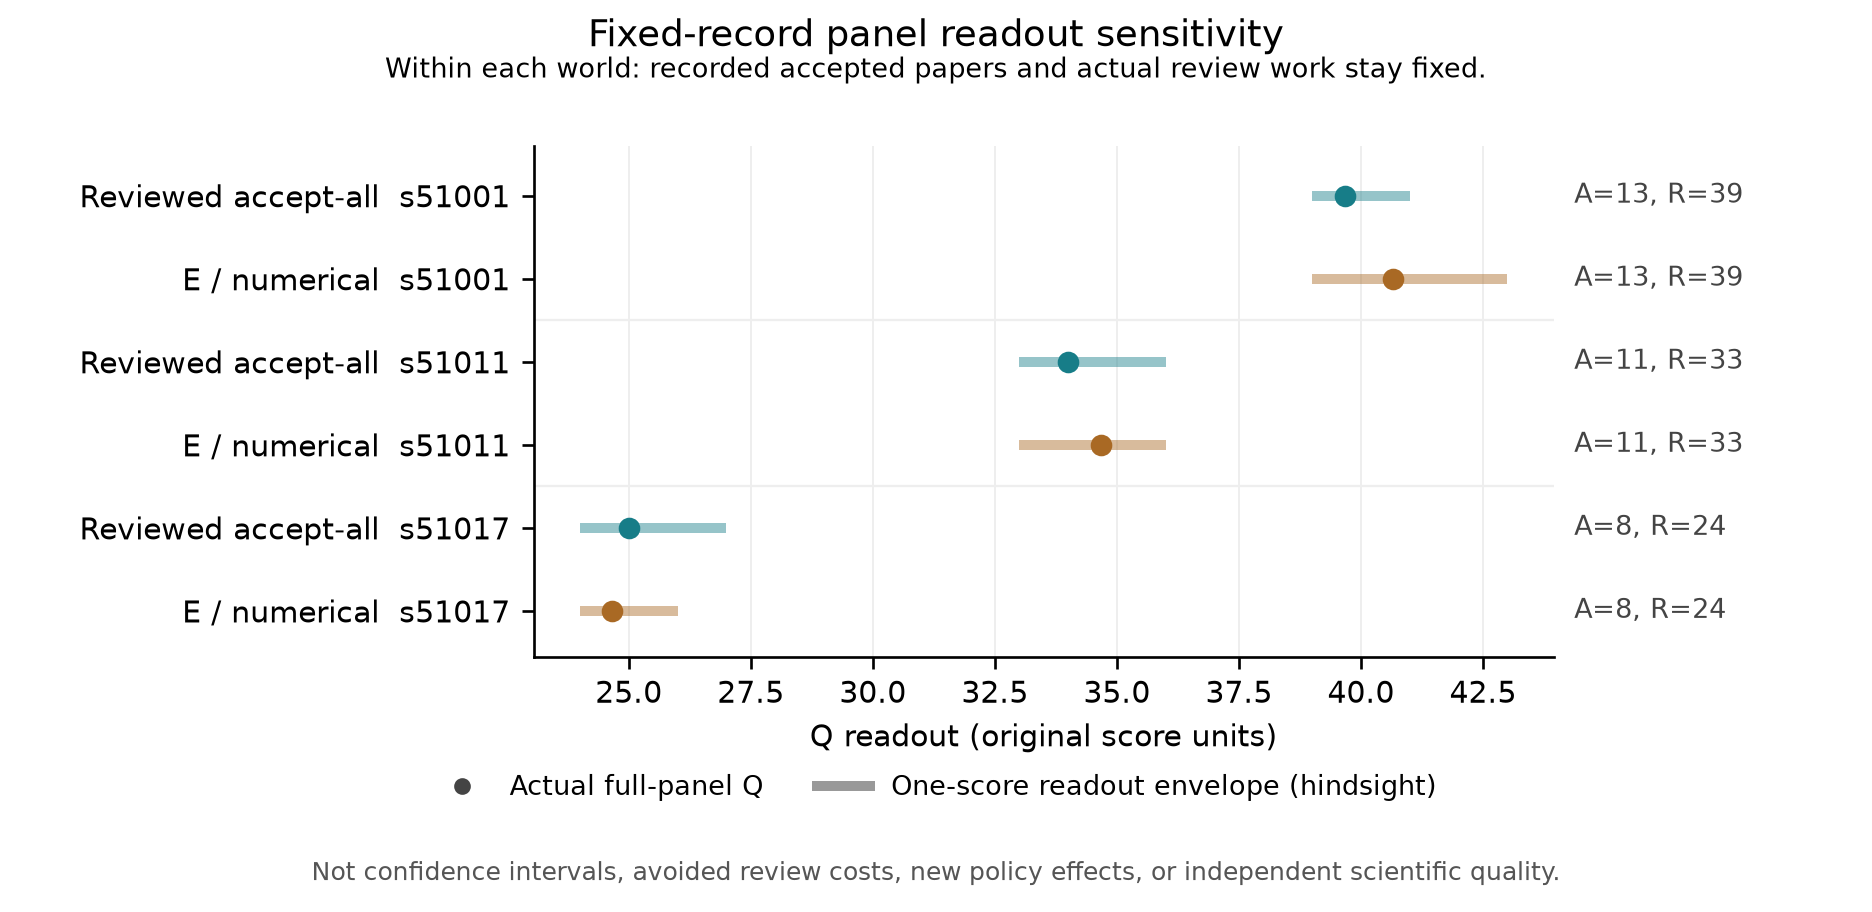
\includegraphics[width=\linewidth]{figures/native-panel-sensitivity-v1/fixed-panel-readout.png}
\caption{\textbf{Recorded panel readout sensitivity.} Dots are actual full-panel
Q; bars reuse one score per already reviewed accepted decision, with hindsight
endpoints. Actual A and R remain unchanged. This is not a reviewer-routing
intervention, reduced review cost, new optimization or scientific quality.
Both original-source analyses and both PNG/SVG builds reproduce identically.}
\label{fig:fixed-panel-readout}
\end{figure}

The practical implication is to name the optimization target precisely.
T/E remain legitimate declared proxies; this diagnostic adds no new loss,
fairness condition or adoption veto. A separate blind evaluator could measure
another fixed-panel opinion, but would not itself verify scientific truth.
Claims about knowledge gain would require an independently justified
measurement or actual verification activity within an extension of the native
researcher world. The prospective routing-authority closed-loop study has its
own finite protocol; its in-progress observations are not counted here as a
completed comparison.
\FloatBarrier
